
%%
\newcommand{\BaryImg}[2]{{\includegraphics[width=.095\linewidth,trim=18 160 18 160,clip]{2d-bary/barycenter-#1-#2}}}
\newcommand{\BaryImgLine}[1]{%%%
\BaryImg{#1}{1}&\BaryImg{#1}{2}&\BaryImg{#1}{3}&\BaryImg{#1}{4}&\BaryImg{#1}{5} %%%
}
%%
\newcommand{\BarySurf}[2]{{\includegraphics[width=.095\linewidth,trim=25 10 25 10,clip]{mesh-bary/barycenter-#1-#2}}}
\newcommand{\BarySurfLine}[1]{%%%
\BarySurf{#1}{1}&\BarySurf{#1}{2}&\BarySurf{#1}{3}&\BarySurf{#1}{4}&\BarySurf{#1}{5} %%%
}
%%

%%%%%%%%%%%%%%%%%%%%%%%%%%%%%%%%
%%
\begin{figure*}\centering
\HighResFig{
%%%%%
\begin{tabular}{@{}c@{}c@{}c@{}c@{}c@{}}
\BaryImgLine{1}\\
\BaryImgLine{2}\\
\BaryImgLine{3}\\
\BaryImgLine{4}\\
\BaryImgLine{5}
\end{tabular}
%%%%%
\hspace{5mm}
%%%%%
\begin{tabular}{@{}c@{}c@{}c@{}c@{}c@{}}
\BarySurfLine{1}\\
\BarySurfLine{2}\\
\BarySurfLine{3}\\
\BarySurfLine{4}\\
\BarySurfLine{5}
\end{tabular}
%%%%%
}{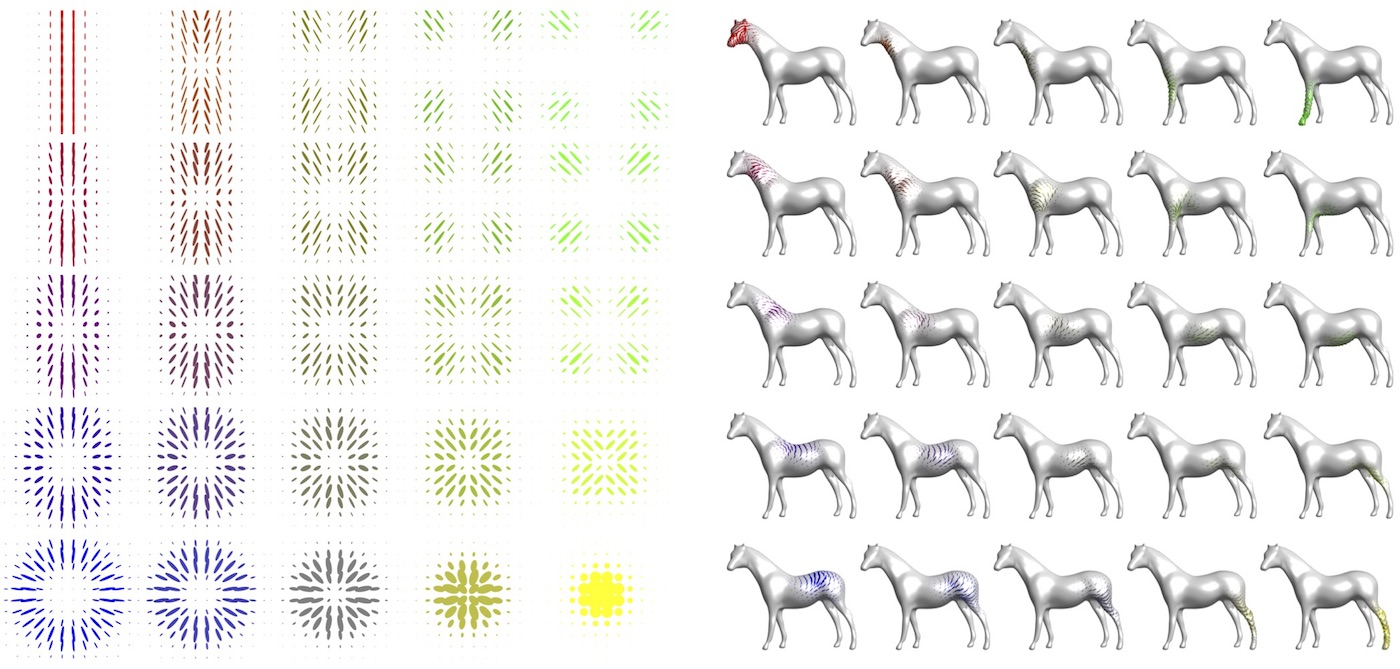
\includegraphics[width=\linewidth]{bary-all}}
\caption{$5 \times 5$ barycenters of four input measures (displayed in the four corners). The weighs $w \in \RR^4$ correspond to bilinear interpolation weights~\eqref{eq-bilinear} inside the square.
} \label{fig:barycenters}
\end{figure*}
%%%%%%%%%%%%%%%%%%%%%%%%%%%%%%%%